%!BIB TS-program = biber
\documentclass[11pt]{article}%
\usepackage{amsmath}
\usepackage{amsfonts}
\usepackage{amssymb,tcolorbox}
\usepackage{graphicx}
\usepackage{amssymb}%
\usepackage{siunitx}
\usepackage{listings}
\usepackage[style=ieee]{biblatex}
\setcounter{MaxMatrixCols}{30}
\providecommand{\U}[1]{\protect\rule{.1in}{.1in}}
\providecommand{\U}[1]{\protect\rule{.1in}{.1in}}
\providecommand{\U}[1]{\protect\rule{.1in}{.1in}}
\newtheorem{theorem}{Theorem}
\newtheorem{acknowledgement}[theorem]{Acknowledgement}
\newtheorem{algorithm}[theorem]{Algorithm}
\newtheorem{axiom}[theorem]{Axiom}
\newtheorem{case}[theorem]{Case}
\newtheorem{claim}[theorem]{Claim}
\newtheorem{conclusion}[theorem]{Conclusion}
\newtheorem{condition}[theorem]{Condition}
\newtheorem{conjecture}[theorem]{Conjecture}
\newtheorem{corollary}[theorem]{Corollary}
\newtheorem{criterion}[theorem]{Criterion}
\newtheorem{definition}[theorem]{Definition}
\newtheorem{example}[theorem]{Example}
\newtheorem{exercise}[theorem]{Exercise}
\newtheorem{lemma}[theorem]{Lemma}
\newtheorem{notation}[theorem]{Notation}
\newtheorem{problem}[theorem]{Problem}
\newtheorem{proposition}[theorem]{Proposition}
\newtheorem{remark}[theorem]{Remark}
\newtheorem{solution}[theorem]{Solution}
\newtheorem{summary}[theorem]{Summary}
\newenvironment{proof}[1][Proof]{\noindent\textbf{#1.} }{\ \rule{0.5em}{0.5em}}
\addtolength{\oddsidemargin}{-.875in}
\addtolength{\evensidemargin}{-.875in}
\addtolength{\textwidth}{1.75in}
\addtolength{\topmargin}{-1in}
\addtolength{\textheight}{2in}
\usepackage{tocloft}
\usepackage{color} %red, green, blue, yellow, cyan, magenta, black, white
\definecolor{mygreen}{RGB}{28,172,0} % color values Red, Green, Blue
\definecolor{mylilas}{RGB}{170,55,241}

\addbibresource{proj2.bib}

\title{MANE 6710 - Numerical Design Optimization Lab 2}
\author{Human 6966}
\date{October 20 2024}

\renewcommand{\contentsname}{Table of Contents:}
\setcounter{tocdepth}{2} % Include sections and subsections
\setlength{\cftbeforesecskip}{0.5cm} % Adjust spacing between entries
\begin{document}
\maketitle
\newpage
\tableofcontents
\newpage
\addcontentsline{toc}{section}{Executive Summery}
\section*{Executive Summery}
\label{sec:abstract}

Wing spars are an important part of aviation design because they support the loading of airplane wings, enabling airplanes to stay in the air. These must be as light as possible as this increases the load capacity of the aircraft, which is an important consideration for most aircraft designs. This lab focuses on choosing and using optimization algorithms in Matlab (\lstinline{fmincon()}) along with the complex stem method of approximating gradients to optimize the profile of a wing spar to minimize their mass. A two-dimensional discretized version of the Euler-Bernoulli Beam Theory was chosen to analyze the structural system, and the SQP algorithm for \lstinline{fmincon()} was selected to optimize the profile of the wing spar. The SQP algorithm was successfully able to minimize the mass of the wing spar within the problem constraints by minimizing the thickness and outer radius of the spar.

\section{Analysis Introduction}
\label{sec:intro}

\subsection {Methodology}
\label{sec:analysismethod}

The method used to analyze the stress in the beam was the Euler-Bernoulli Beam Bending Theory (Equation \ref{eqn:bend}).
\begin{equation}
\label{eqn:bend}
\frac{d^{2}}{dx^{2}}(EI_{yy}\frac{d^{2}w}{dx^{2}})=q, \forall x \in [0,L]
\end{equation}
Where:
\begin{itemize}
\item w: the vertical displacement
\item q(x): the applied load
\item E: the Young's modulus
\item $I_{yy}$: Second-moment of area with respect to the y-axis
\end{itemize}
With the initial conditions:
\begin{itemize}
\item $w(0)=0$: No displacement at the root
\item $\frac{dw}{dx}(0)=0$: No angular displacement at the root
\item $\frac{d^{2}w}{dx^{2}}(L)=0$: No stress at tip
\item $\frac{d^{3}w}{dx^{3}}(L)=0$: No stress at tip
\end{itemize}
Equation \ref{eqn:bend} can be solved for the magnitude of the normal stress (equation \ref{eqn:sigma}).
\begin{equation}
\label{eqn:sigma}
\sigma_{xx}(x)=|-r_{outer}E\frac{d^{2}w}{dx^{2}}|
\end{equation}
This is discretized using the finite-element method, with the solution represented using Hermite-cubic shape functions derived from the minimization of the potential energy function. The distributed load is given by equation \ref{eqn:q} with $q_{L}=0$ and F being the total applied load. 
\begin{equation}
\label{eqn:q}
q(x)=(1-\frac{x}{L})q_{0}+\frac{x}{L}q_{L}, q_{0}=\frac{2*F}{L}-q_{L}
\end{equation}

\subsection{Assumptions}
\label{sec:assumption}
To simplify the physical model and fundamental equations, the following assumptions were made:
\begin{enumerate}
   	 \item Planar symmetry on the logitudinal axis
    	\item Smoothly varying cross section
	\item Plane sections that are normal to longitudinal plane before bending remain normal after bending 
	\item Internal strain energy accounts only for bendding moment deforrmations
	\item Deformations are small enough that nonlinear effects are negligible
	\item Carbon fiber is an elastic and isotropic material and has the following propeties:
	\begin{enumerate}
	\item E=70 GPa
	\item $\sigma_{ultimate}$=600 MPa
	\item $\rho$=1600 kg/m$^{3}$
	\end{enumerate}
\end{enumerate}

\subsection{Limitations}

These assumptions limit this analysis method to static systems with radial symmetrical cross-sections. Additionally, though it is assumed to be an isotropic material to simplify the model, composites like carbon fiber are highly anisotropic meaning the loading direction has a significant impact on the physical properties of the material (like the Young’s modulus), resulting in a large error in the results. Additionally, the assumption that nonlinear effects are negligible is only viable for the elastic region of loading (yield stress). As many of these conditions would not be met in the real world, there is expected to be significant error in the result of this analysis

\section{Parameterization of the Geometry}
\label{sec:parameterization}

The shape of the wing spar was defined by linear interpolation between the inner and outer radii of adjacent nodes.
\begin{equation}
r_{in}(x^{*})=(1-x)*r_{in}(i)+x*r_{in}(i+1), i=floor(\frac{N*x^{*}}{L}) ,  x=\frac{x^{*}}{L}
\end{equation}
\begin{equation}
r_{out}(x^{*})=(1-x)*r_{out}(i)+x*r_{out}(i+1), i=floor(\frac{N*x^{*}}{L}) ,  x=\frac{x^{*}}{L}
\end{equation}
These equations were then descritized into a two-dimensional mesh.

\section{Optimization Method and Limitations}
\label{sec:optimizationmethod}
The SQP (Sequential Quadratic Programming) Algorithm was chosen for \lstinline{fmincon()} (Matlab's nonlinear optimization problem solver \cite{matlab}) to solve the minimization problem. The SQP algorithm uses a quasi-Newton update method to approximate the Hessian, which is used to solve the quadratic subproblems, which are linearized around the current state. Then the algorithm does a line search to determine the step size in the direction of the solution for each node in the mesh. The algorithm iterates through the updated states until the solutions to the quadratic subproblems converge into a smooth gradient. To perform this analysis, the following assumptions were made:
\begin{enumerate}
	\item Constraints are continuously twice differentiable
	\item The objective function is continuously twice differentiable
	\item There is a 'good' initial guess
	\item There is a 'good' mesh
\end{enumerate}
The methodology and assumptions impose the following limitations on this analysis method:
\begin{enumerate}
	\item Due to the derivative assumptions, smooth objective  and model functions are required
	\item Due to ending conditions, a smooth mesh is required
	\begin{itemize}
		\item No discontinuities can be in the mesh
		\item The mesh must be fine enough to capture the gradient 
	\end{itemize}
	\item Due to the gradient-driven update method, the solution may not recover from a step outside the constraints
	\begin{itemize}
		\item Initial guess should start solver inside constraints (algorithm may or may not work otherwise)
		\item A 'bad' step can put algorithm outside constraints
	\end{itemize}
	\item The algorithm won't know if the minimum it found is a local or global minimum 
	\item If the objective function behavior cannot be adequately captured in a localized linear model, this can create ’bad’ steps due to deviation between actual and linearized models
\end{enumerate}

The complex step method was used to generate the gradients for fmincon for the nonlinear constraint and the objective functions using equation \ref{eqn:del}, and the nonlinear stress constraint given by equation \ref{eqn:c}.
\begin{equation}
\label{eqn:del}
\frac{df}{dx}\approx\frac{imag(f(x+hi)))}{h}, h=1e-30
\end{equation}
\begin{equation}
\label{eqn:c}
c(i)=\frac{\sigma}{\sigma_{ultimate}}-1\leq0
\end{equation}

\section{Optimization Problem}
\label{sec:problem}
The objective of this lab is to apply the principles learned in lecture to optimize the shape of a wing spar modeled within the following criteria and constraints\cite{lab2doc}:
\begin{enumerate}
	\item The design is to be two-dimensional 
	\item Has a width of L = 7.5m 
	\item The spar should survive under 2.5gs of acceleration ($F=2.5*\frac{m}{2}*9.81$)
\end{enumerate}
The objective of this project is to optimize the shape of the wing spar to minimize the weight. The model geometry was parameterized and discretized (see section \ref{sec:parameterization} for more details) and applied to a discretized version of the Euler-Bernoulli Beam Theory to analyze the problem. The method chosen for the minimization problem was the SQP algorithm for the fmincon Matlab function (see section \ref{sec:optimizationmethod} for more details) with the gradients calculated using the complex step method.
\section{Results}
The convergence plot shown in Figure \ref{fig:conv} was calculated for the stress at the spar tip with an initial shape function r(x). The plot shows an exponential decrease towards 0 as the number of segments increases. This behavior makes sense because as the number of variables increases, the error from the volume and discretization calculations decreases. The acceptable number of elements was calculated as 50 as it represented a 6.5 orders of magnitude decrease from the maximum normalized stress while also not resulting in a long run time, which is similar to the conditions for the first-order optimality of the iteration solutions.
\begin{figure}[h!]
    \centering
    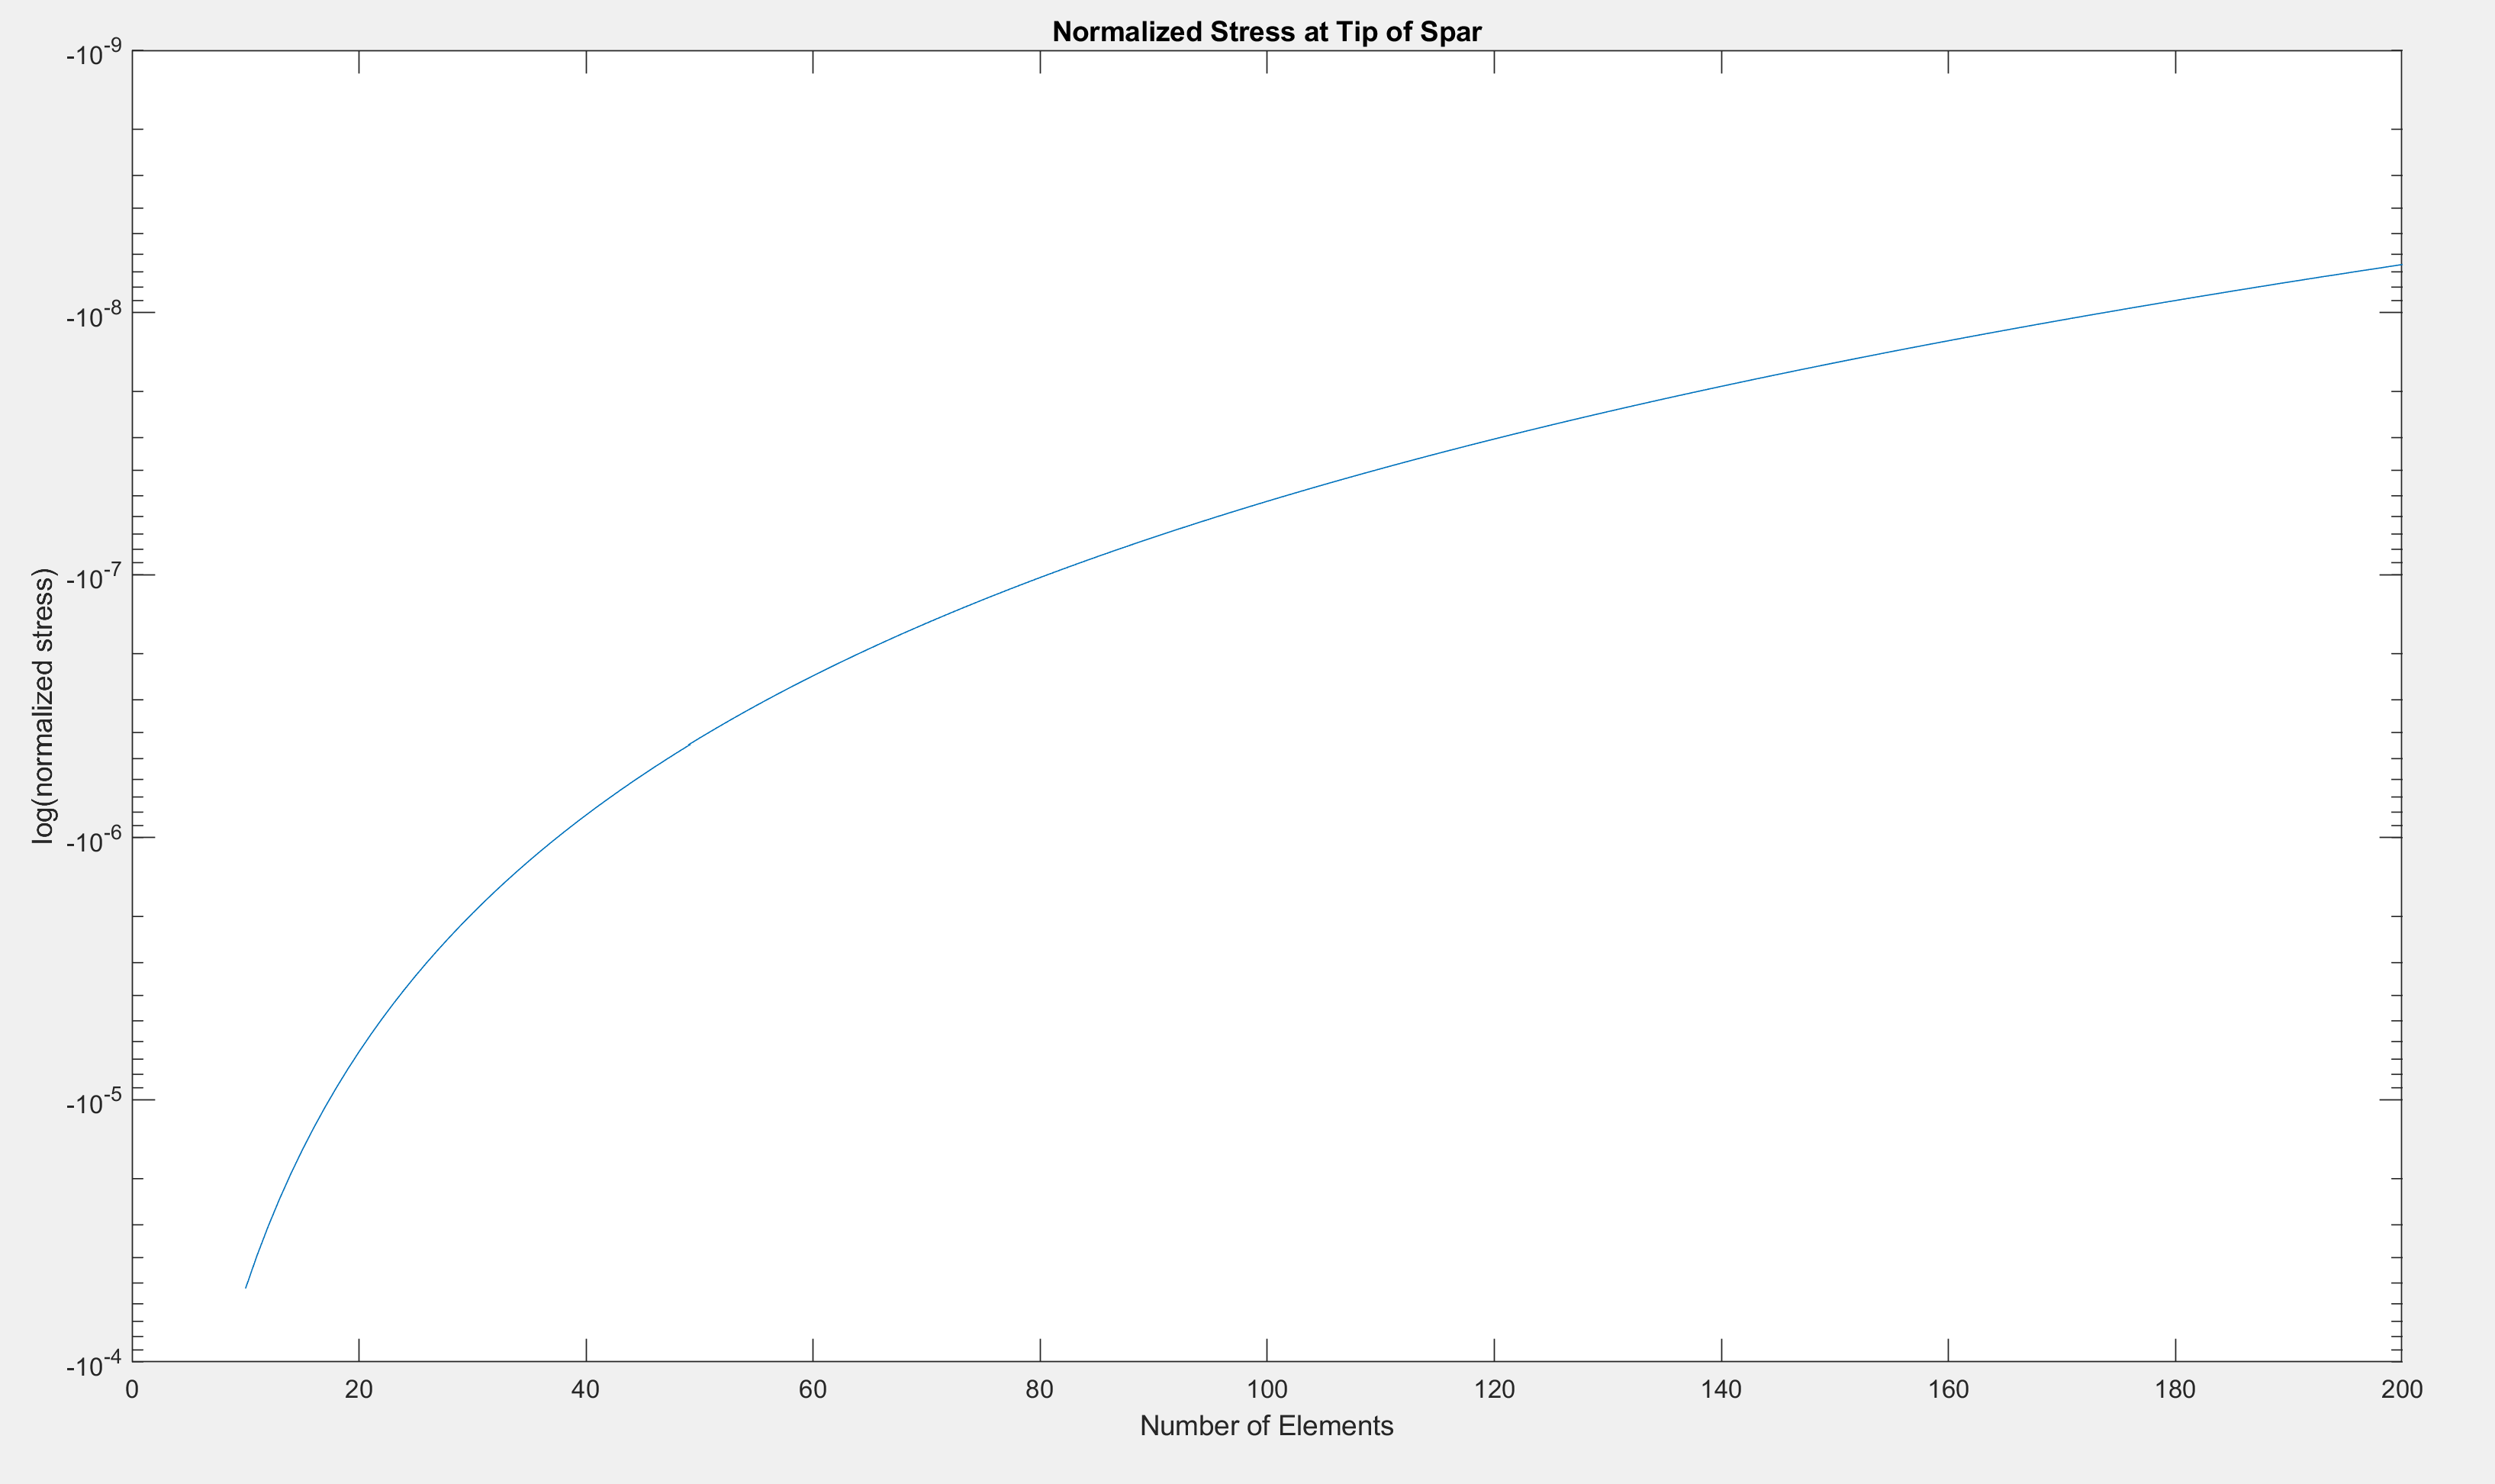
\includegraphics[width=0.75\linewidth]{convergence.png}
    \caption{ Plot of the  stress vs N }
    \label{fig:conv}
\end{figure}

The optimized shape of the wing spar with the chosen parameterization and number of elements (50) is shown in Figure \ref{fig:cross}. This result makes sense because it shows a similar inner and outer radii to the provided nominal design which gets thinner before the outer radii decrease until the design hits the lower bound of the design space, which would result in a limited mass of the spar

\begin{figure}[h!]
    \centering
    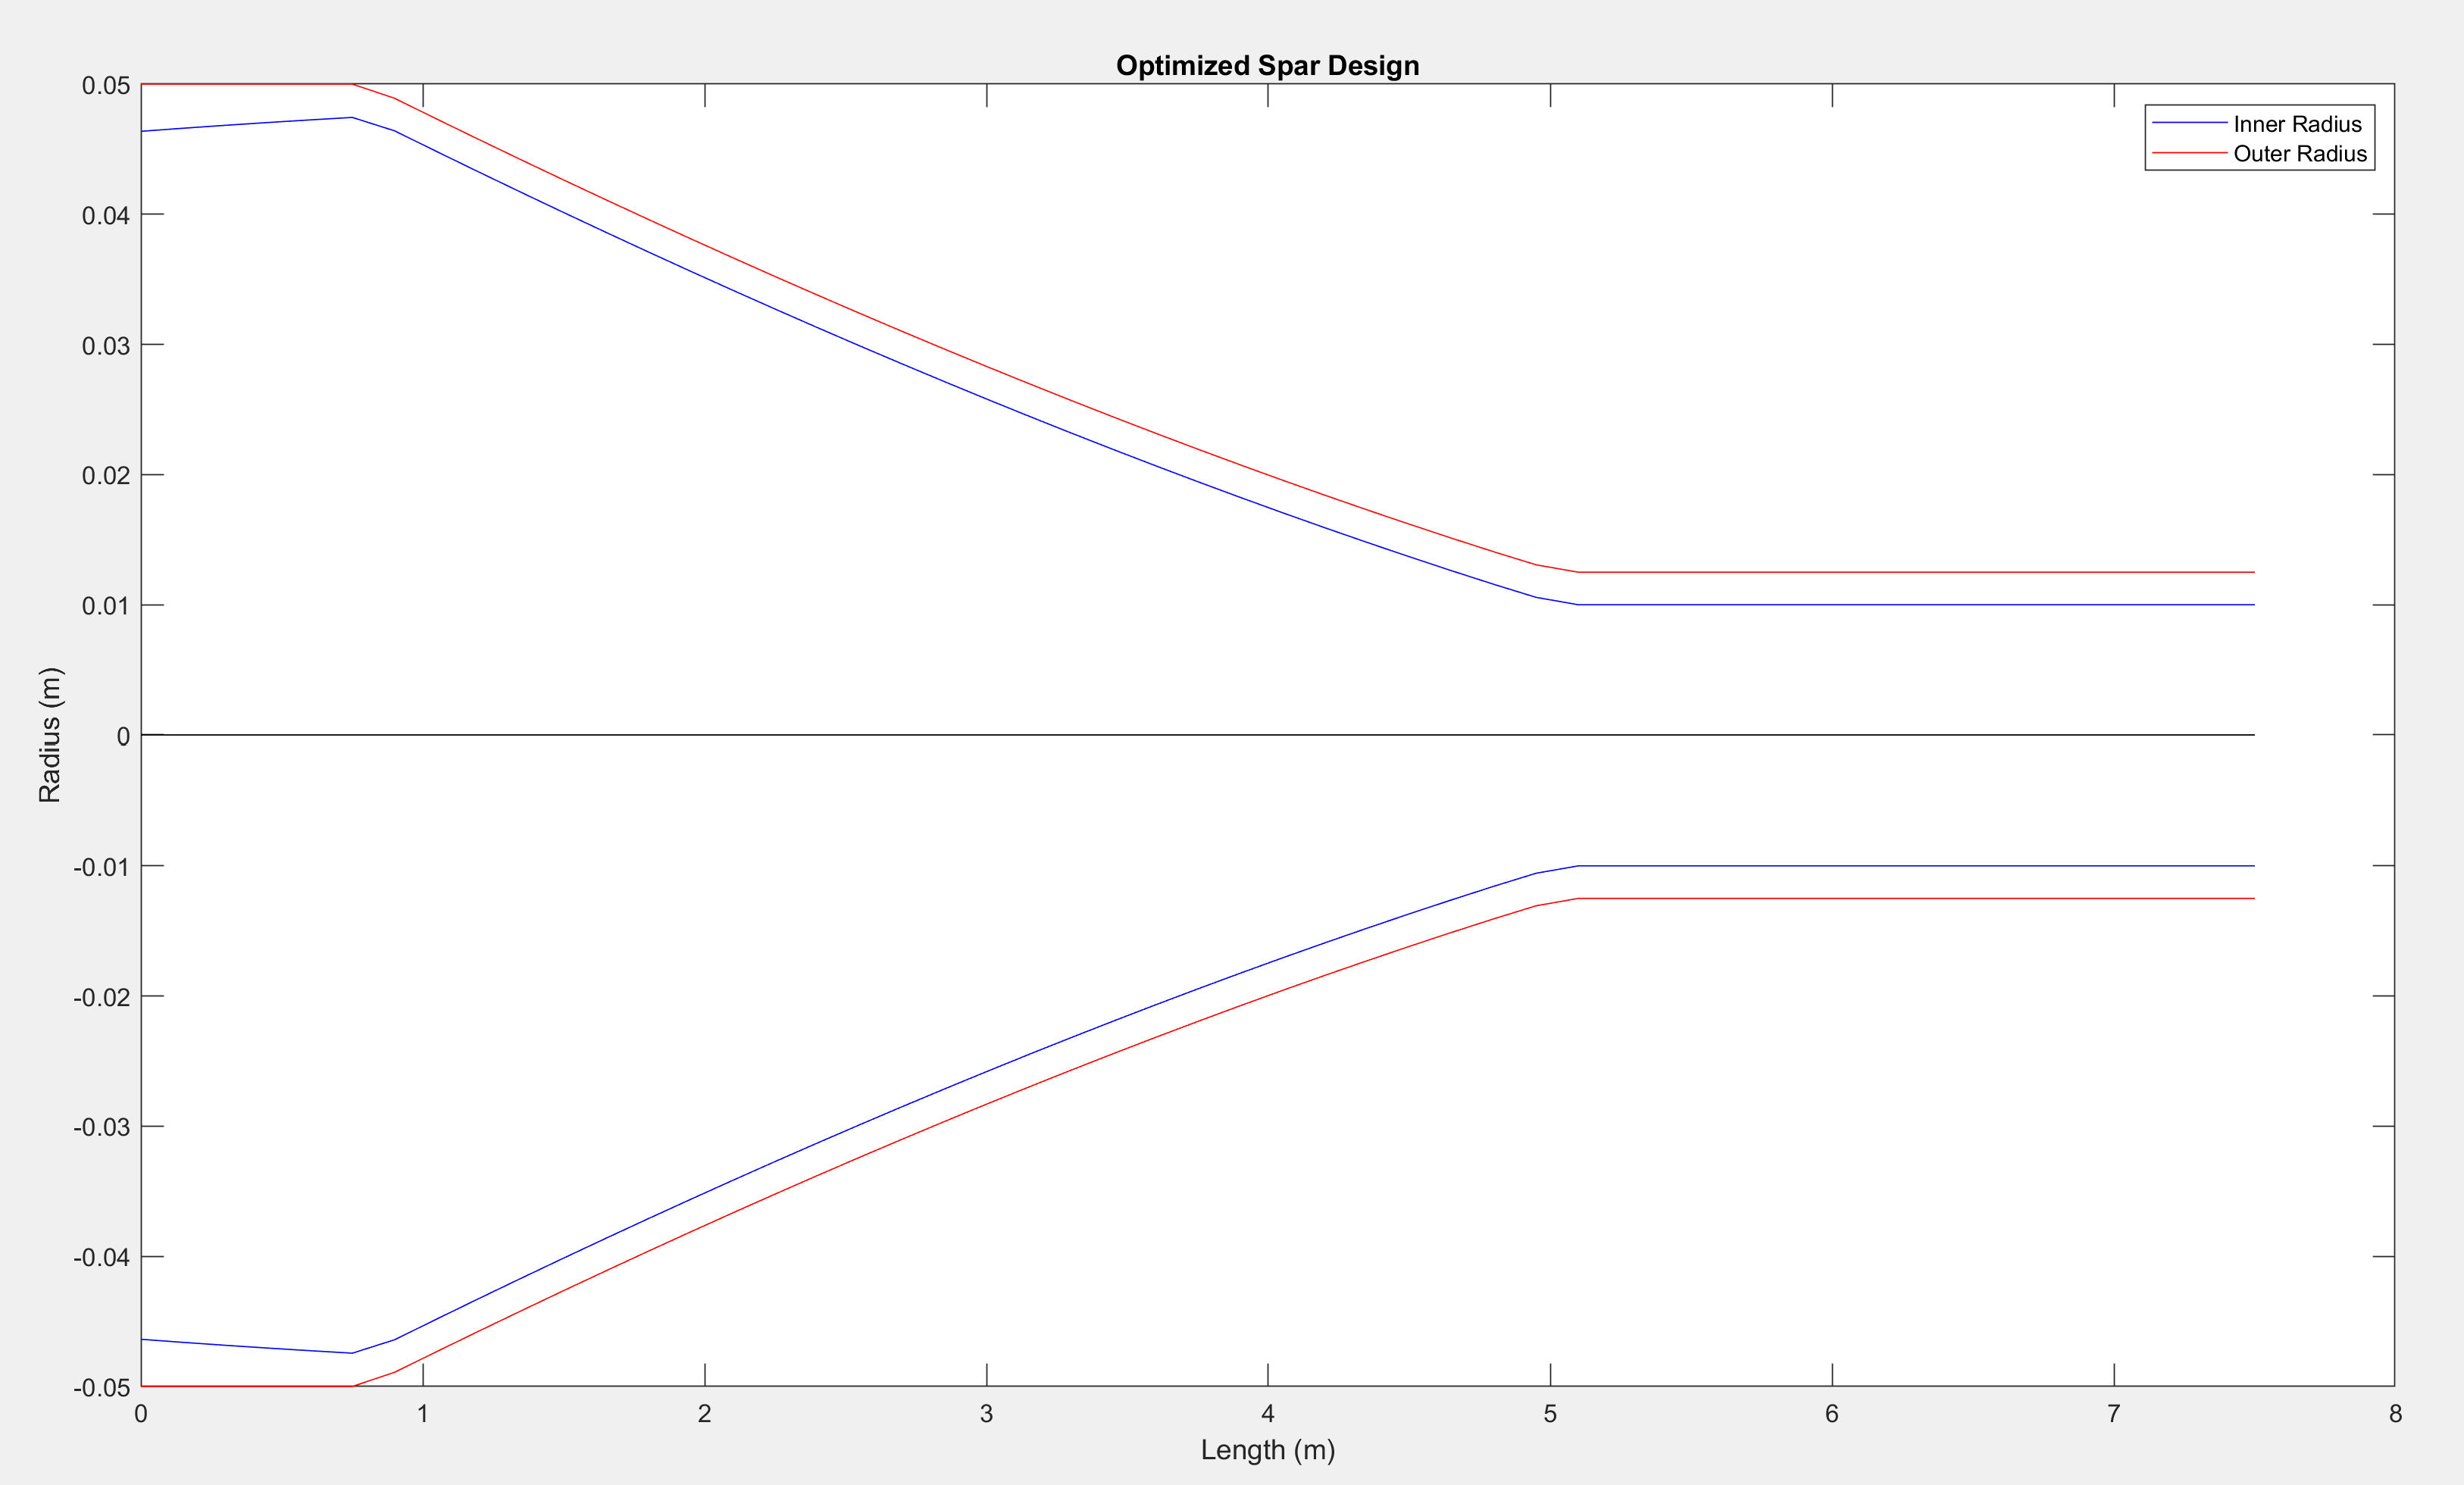
\includegraphics[width=0.75\linewidth]{fmiconoutput.png}
    \caption{ Plot of the Wing Spar Cross Section }
    \label{fig:cross}
\end{figure}
\newpage
The feasibility graph shows that the feasibility score of the current solution decreased rapidly over the first iteration and then stabilized over the remaining iterations as the First-Order Optimality improved. The First-Order Optimality graph shows a slow improvement over the iterations until the solver converged on a minimum causing a rapid improvement (see Figure \ref{fig:feas} both Feasibility and First Order Optimality decreased by sixteen orders of magnitude over the iterations). (Note: the feasibility score for both the general and complex step method spends most of the optimization at 0, so the semilog plot didn't work for them see \ref{fig:feas2} for the semi-log plot of the first order optimization).

\begin{figure}[h!]
    \centering
    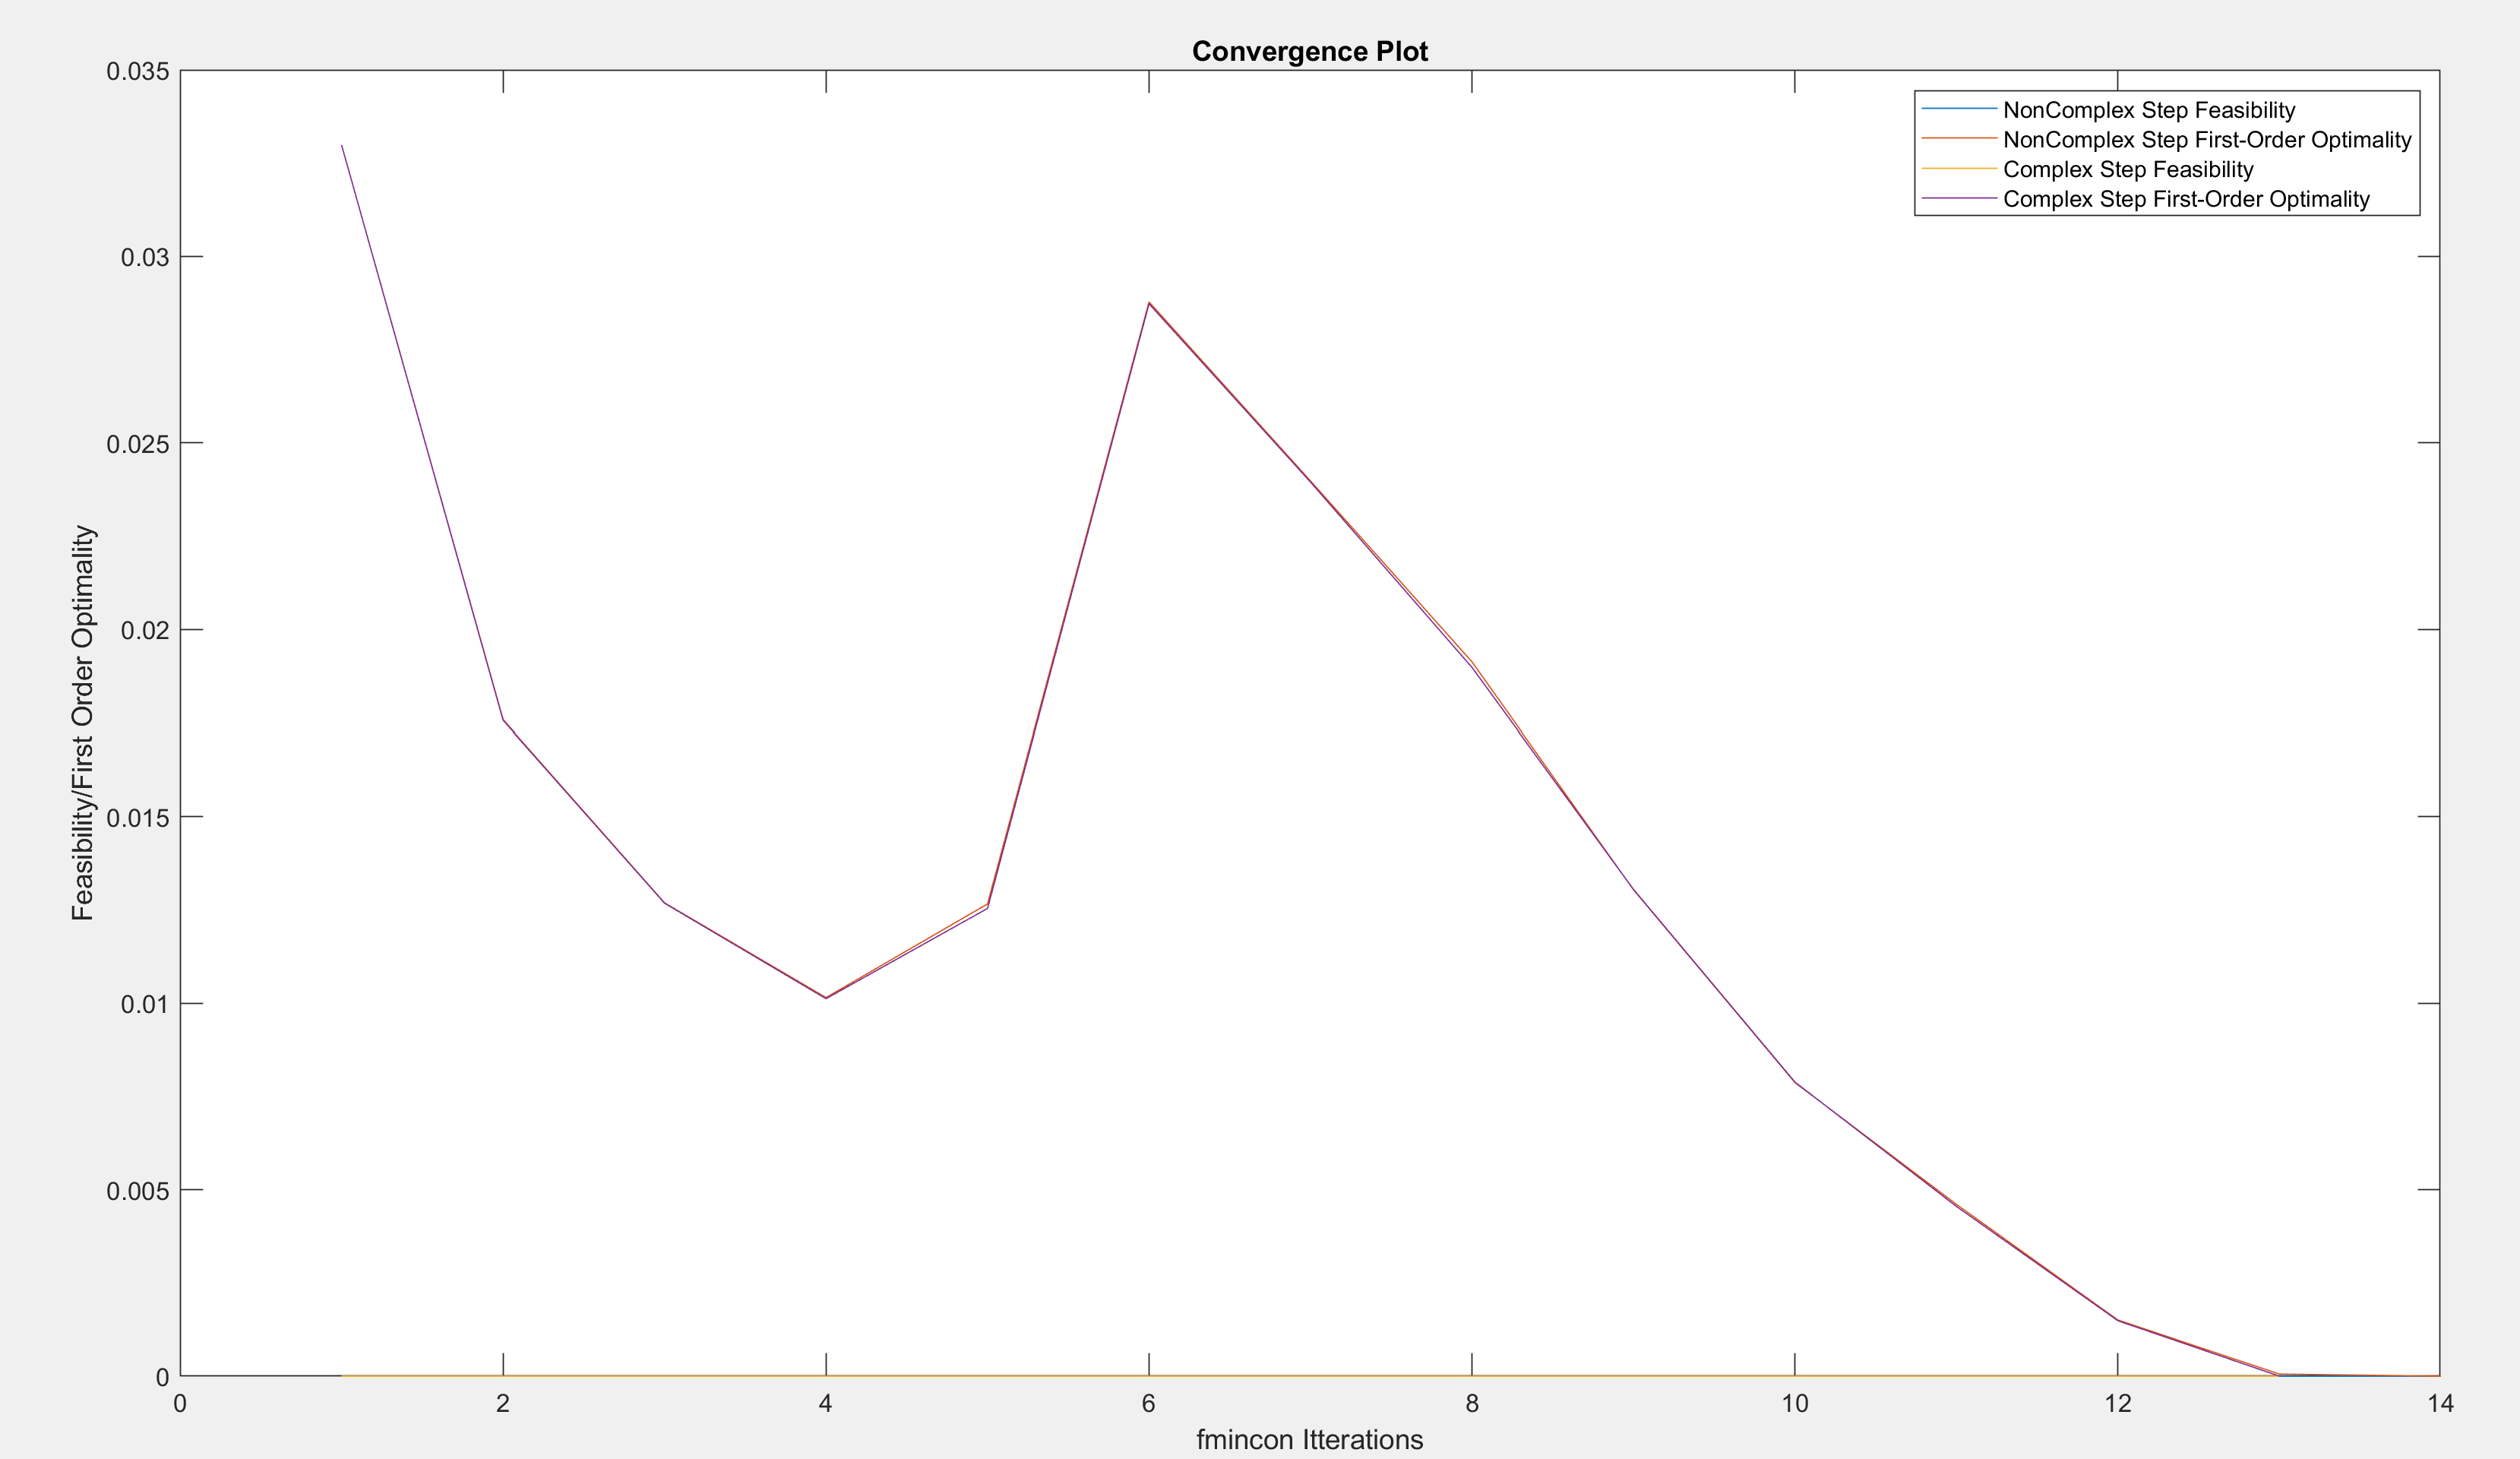
\includegraphics[width=0.75\linewidth]{feas.png}
    \caption{ The Feasibility and Convergence Plots }
    \label{fig:feas}
\end{figure}
\begin{figure}[h!]
    \centering
    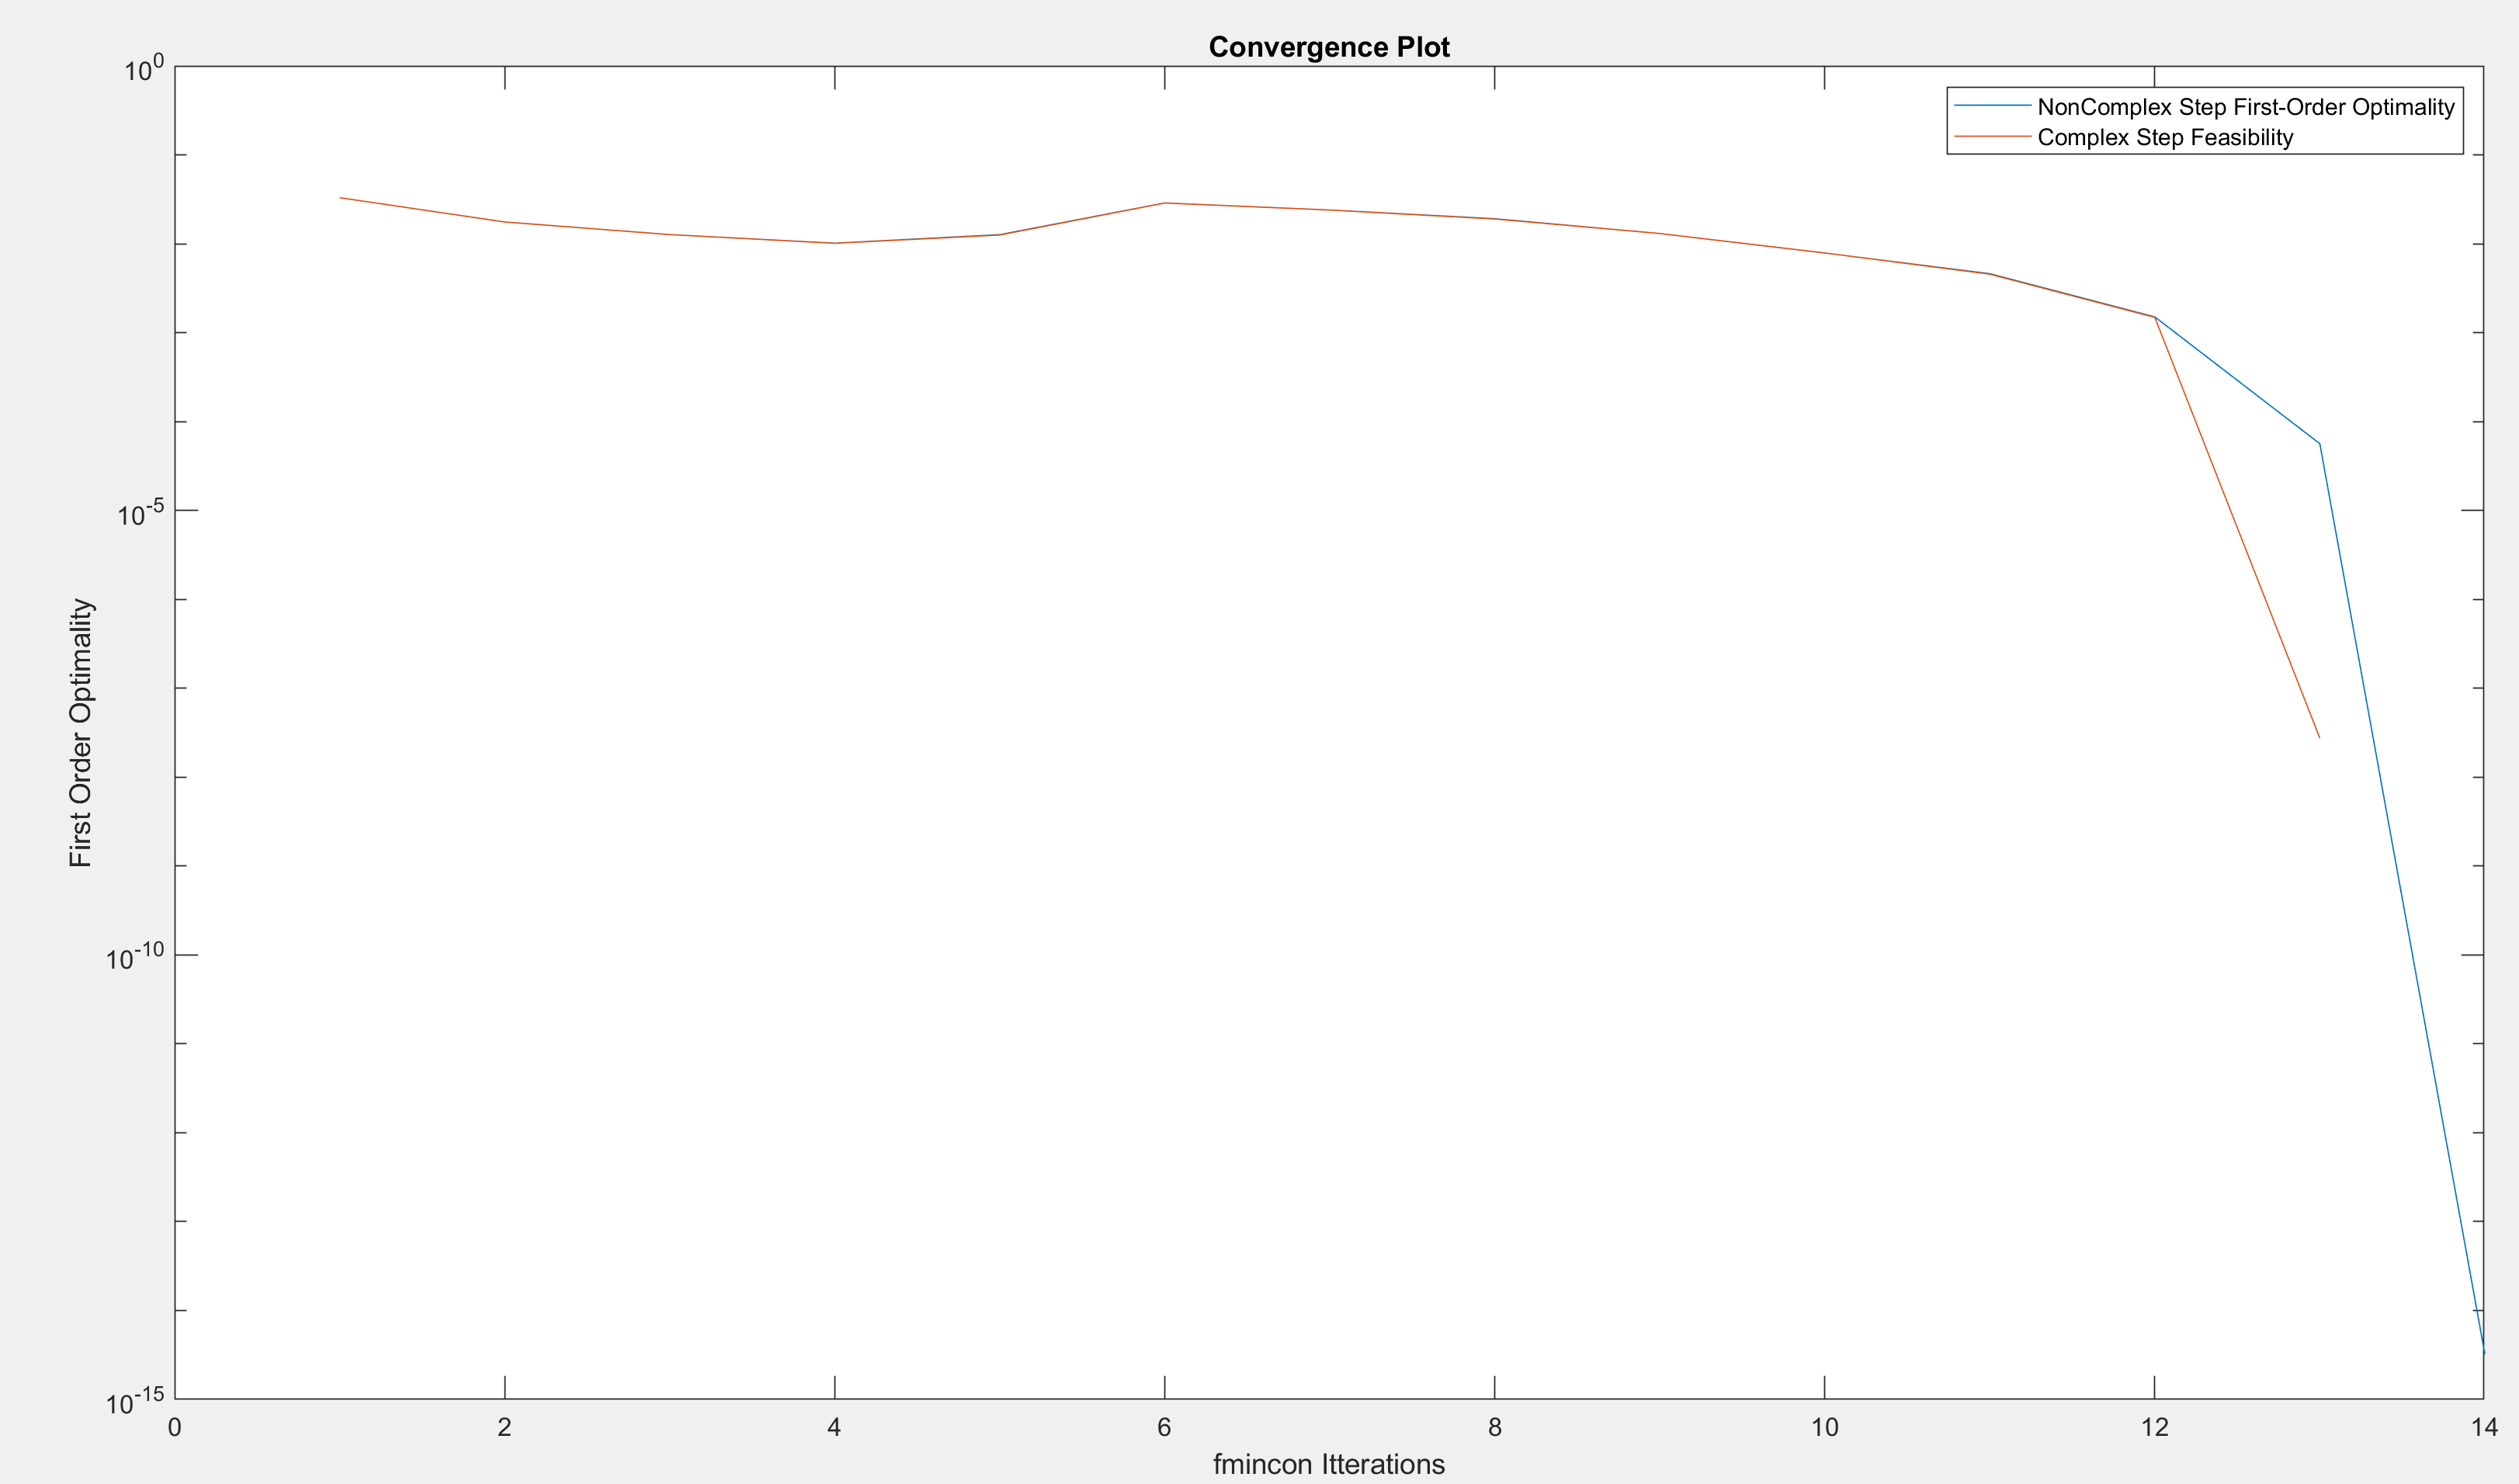
\includegraphics[width=0.75\linewidth]{converg.png}
    \caption{ The Convergence Plots }
    \label{fig:feas2}
\end{figure}
\medskip

\section{Conclusions}
The implementation of the SQP optimization algorithm with the complex step gradient method for this lab was successful. The resulting shape function for the optimized wing spar section profile made sense because it minimized the mass by minimizing the thickness and outer radius of the spar. The resulting calculated mass from the optimized wing spar was less than forty percent of the baseline design ($.4*13.26=5.3020 > 5.0707 $ kg) while remaining within the problem constraints. Complex step and the normal fmincon optimizations resulted in the same optimized design with the complex step method running noticeably faster, especially when a higher number of elements was used.

 Basic optimization algorithms, such as the ones used in this lab, can be powerful tools for understanding the complex interactions between different design variables in engineering design problems and balancing the design variables to arrive at an optimal solution. Understanding how these algorithms work and the trade-offs between accuracy and run time shown in the convergence study is important when utilizing these algorithms to solve problems. 

\addcontentsline{toc}{section}{References}
\printbibliography
\newpage
\section{Appendix}

\lstset{language=Matlab,%
    %basicstyle=\color{red},
    breaklines=true,%
    morekeywords={matlab2tikz},
    keywordstyle=\color{blue},%
    morekeywords=[2]{1}, keywordstyle=[2]{\color{black}},
    identifierstyle=\color{black},%
    stringstyle=\color{mylilas},
    commentstyle=\color{mygreen},%
    showstringspaces=false,%without this there will be a symbol in the places where there is a space
    numbers=left,%
    numberstyle={\tiny \color{black}},% size of the numbers
    numbersep=9pt, % this defines how far the numbers are from the text
    emph=[1]{for,end,break},emphstyle=[1]\color{red}, %some words to emphasise
    %emph=[2]{word1,word2}, emphstyle=[2]{style},    
}
\subsection{getq.m}
\label{sec:getq}
\lstinputlisting{code/getq.m}
\newpage
\subsection{run.m}
\label{sec:run}
\lstinputlisting{code/run.m}
\newpage
\subsection{getR.m}
\label{sec:getR}
\lstinputlisting{code/getR.m}
\newpage
\subsection{getI.m}
\label{sec:getI}
\lstinputlisting{code/getI.m}
\newpage
\subsection{getC.m}
\label{sec:getC}
\lstinputlisting{code/getC.m}
\newpage
\subsection{putR.m}
\label{sec:putR}
\lstinputlisting{code/putR.m}
\newpage
\subsection{calcVol.m}
\label{sec:calcVol}
\lstinputlisting{code/calcVol.m}
\newpage
\subsection{plots.m}
\label{sec:plots}
\lstinputlisting{code/plots.m}
\subsection{fmincon Output}
\label{sec:fincon}
\begin{figure}[h!]
    \centering
    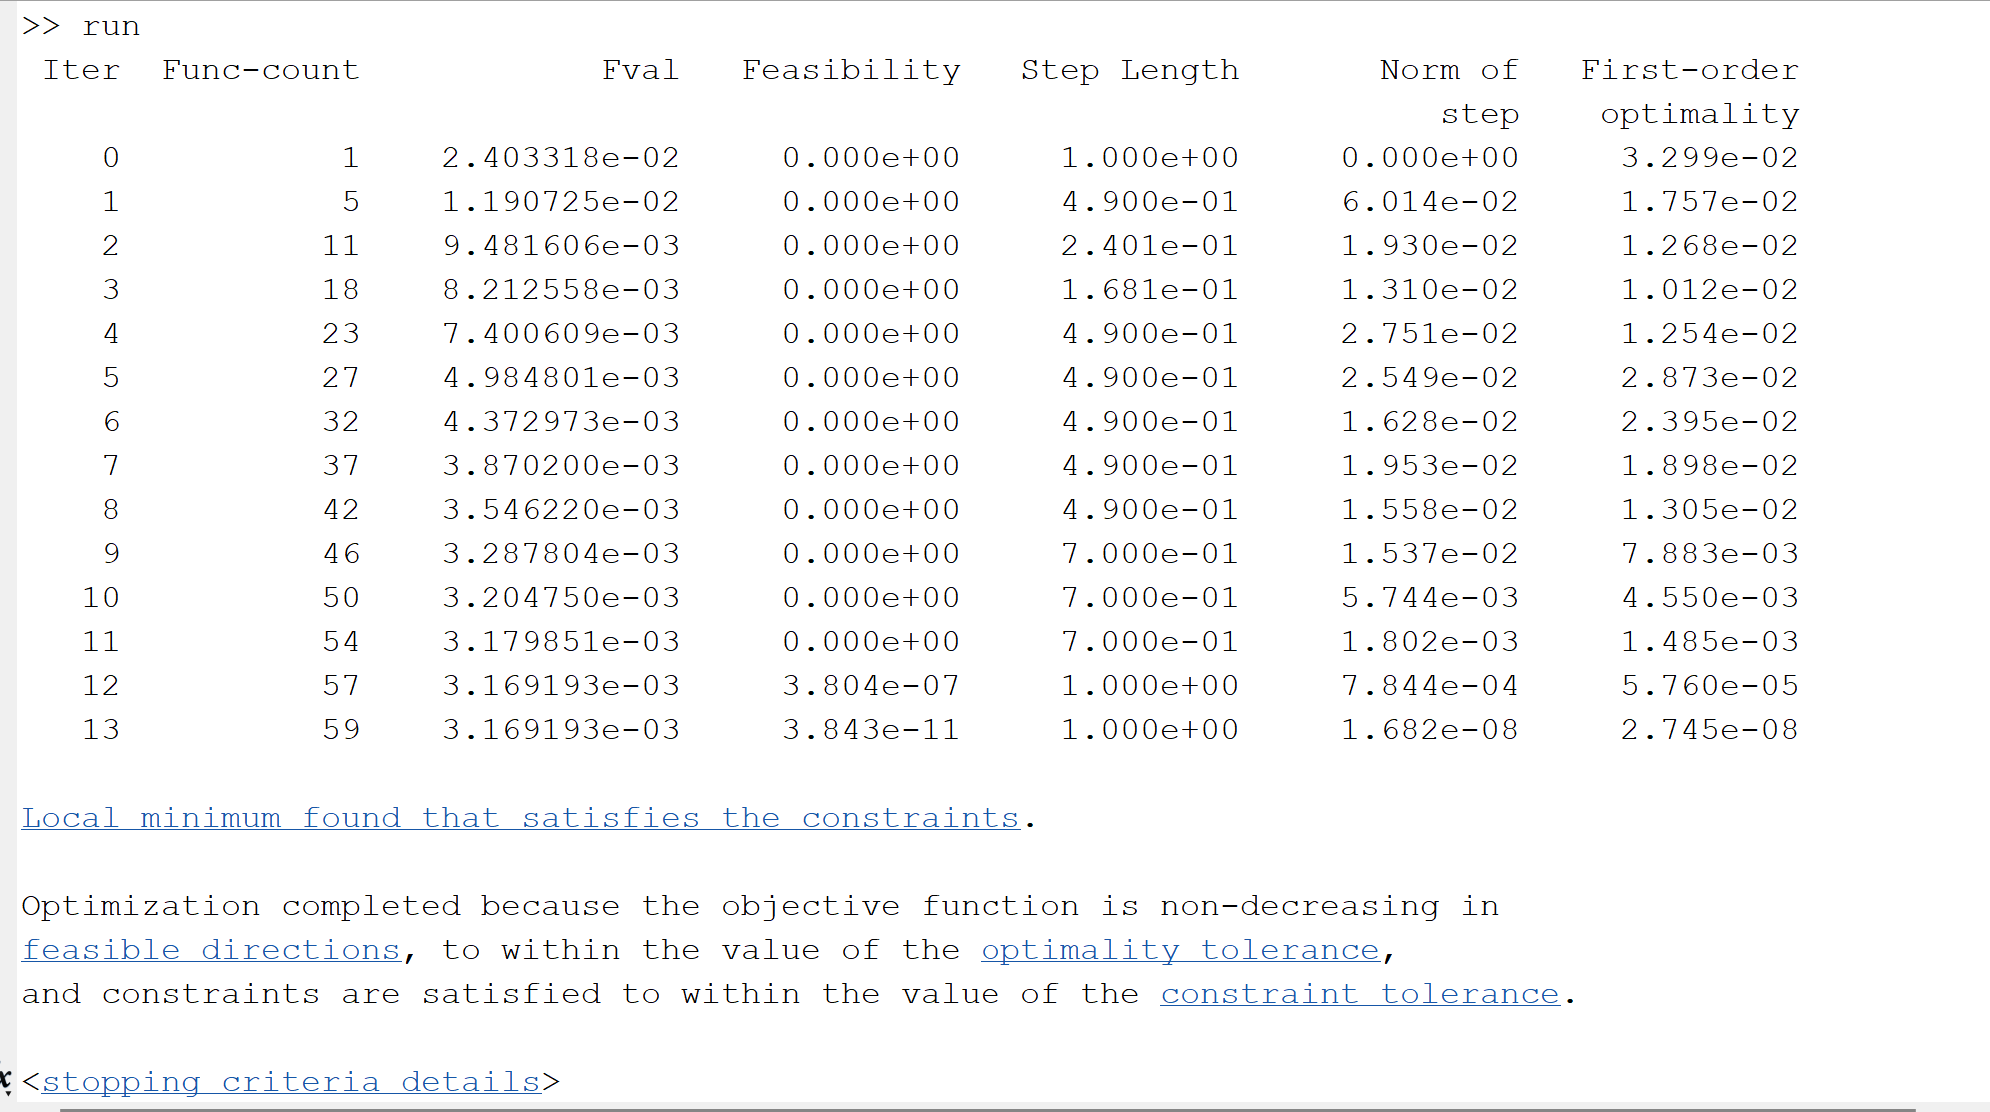
\includegraphics[width=0.75\linewidth]{fminconoutput.png}
    \caption{ The Outpt of fmincon }
    \label{fig:fmincon}
\end{figure}

\end{document}